%!TEX root = ../Masterthesis.tex
\chapter{Tracking in real space}
The previous sections provided information on the structure of the human hand and how to represent it in the digital space. To apply the algorithms presented in Section \ref{sec:kinematics} to our digital hand model, we need input data from our real world representative.
\section{General tracking technologies}
\label{General tracking technologies}
The methods for gaining positional data can be roughly categorized into two major groups, glove based methods and vision based methods. Glove based methods have already been in developement since the 1980's \cite{Bolt.1980} and since then have resulted in several solution attempts. Sturman and Zeltzer gave a survey on the existing tracking methods in their paper \cite{Sturman.1994}. They distinguish between two areas of tracking, first the 3D positional tracking of the hand (and also other bodyparts) without regard to the hands shape and secondly the tracking of the hand shape with glove technologies. These tracking technologies presented are still applied today in modern tracking solutions \cite{Welch.2002,Rolland.2001}. They account for solutions with optical tracking based on marker detection, magnetic detection via measurements of an artificial magnetic field \cite{Raab.1979} and acoustic measurements via triangulation of ultrasonic pings.

\subsection{Optical tracking}
The components for an optical tracking systems consist of several cameras for object detection and a tracking characteristic of the object to be tracked. These characteristics can either be artificially applied ones like active flashing infrared LED on key tracking positions of the body or infrared reflective markers. A series of cameras positioned around the tracking subject will track these markers inside their visual fields. \\The second method uses a single camera to capture the silhouette image of the subject, which is analyzed to determine positions of the various parts of the body and user gestures.\\
The image data is handed over to special software, which correlates the marker positions in the multiple viewpoints and uses the different lens perspectives to calculate a 3D coordinate for each marker. These image interpretation and correlation tasks require computationally costly operations. The marker tracking is also prone to errors through variation in lighting of the scene, material reflection properties and also marker occlusion as the trackers are moved. Also most of the systems rely on several tracking cameras for a complete coverage of the tracking space. This leads to a higher system complexity in terms of setup and calibration.
\begin{figure}[H]
\label{optic reflector tracking}
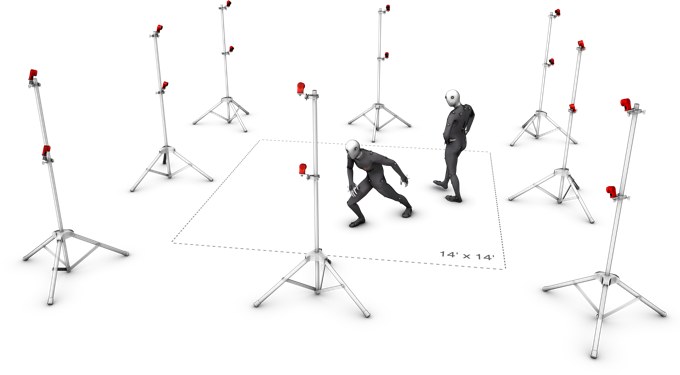
\includegraphics[scale=0.6]{images/flex13MocapVolume.png} 
\caption{Example for an optical tracking system with passive infrared reflector markers \cite{optitrack.2017}}
\end{figure}
\subsection{Magnetic tracking}
The usage of a magnetic field for position tracking is a relatively uncomplicated technology. The earth already provides us with a magnetic field to orient on. Similar to the optical trackers, magnet field sensors can be placed at key tracking positions. These sensors measure field strength in 3 orthogonal oriented axes to produce a 3D vector of the units orientation with respect to the excitation. As the earths magnetic field is prone to changes based on geographical location, data corrections have to be applied to the measurements.\\\\Another solution is to generate an local magnetic field via a multi-coil source unit \cite{Raab.1979}. The source unit coils are energized in sequence and the corresponding magnetic field vector is measured in the sensor unit. With three such excitation's, one can estimate the position and orientation of the sensor unit with respect to the source unit. The downside of this technology is that ferromagnetic and conductive material in the surrounding environment will have an effect on the generated magnetic field. These distortion effects will form small unwanted secondary source units through the induction of small \textit{Foucault currents} from the main sources magnetic field.\\
Magnetic fields have an inverse cubic falloff as a function of distance from the source, which limits the range of operation for the system.
Position resolution in the radial direction from source to sensor depends on the gradient of the magnetic field strength, and thus the positional jitter grows as the fourth power of the separation distance.
In comparison to other tracking technologies, the magnetic field tracking solution has the advantage of not suffering from line of sight problems from tracker occlusion. The magnetic fields are capable of passing through the human body. Also the sensor size for measuring magnetic fields is rather small, giving the trackers a small volume. Furthermore, only one source unit is needed for the tracking of multiple sensor units.
\newpage
\subsection{Acoustic tracking}
The principles of acoustic tracking are very similar to those of optic tracking technologies. Instead of using light waves, the systems utilize acoustic pulses of ultrasonic wavelengths to measure the time of flight between emitter and sensor for range measurement. To get a good measuring result from the systems, the used acoustic transducers have to be as omnidirectional as possible, so that the signal can be detected no matter how the emitter is positioned or oriented in the tracking volume. For the speakers to achieve a wide beam width, their size has to be small.\\
To be able to build the microphones into the tracker, they can only have active surfaces of a few millimeters in diameter. This leads to a reduction in range as the efficiency of acoustic transducers is proportional to the active surface area. Also acoustic systems may have problems with ambient noises occluding the signal. \\This becomes even more critical when using such a system outdoor. Sound waves travel at a much slower speed than light waves which brings benefits and downsides with it. Sound waves can be reflected from objects, producing echos which arrive at the receiving sensor at a later point in time. Here the slower speed can be beneficial as the system can await the first sound occurrence to arrive at the sensor and filter out all later reflections from the data. The reflections of the previous pulse also have to be subsided before a new measurement can be made, lowering the update rates of the system. The air the sound waves travel through is also a limiting factor like humidity, air pressure and air currents can influence the traveling sound waves. In comparison to the optical systems, the acoustic systems are not as prone to occlusion errors since sound waves have a better ability to bend around obstacles than light waves.
Most of these downside can be adressed with a combination of these systems with another form of tracking like in \cite{Foxlin.1998}.
\section{Hand tracking systems}
\label{hand-tracking_systems}
In comparison to the tracking of the whole human body, the tracking of the human hands with their maximum of 27 DOF's each in a small space is rather difficult to handle.
The systems that try to achieve this have to encounter several difficulties. Self occlusion plays a great role in the system design, especially when working with only one optical tracking system for reduced complexity.  These systems need to maintain a certain amount of processing speed for achieving a fluent reproduction of the captured motion. This requires the capability of processing large amounts of data in very short time intervals. Most prototype testing for the described systems is done in an controlled environment with a well known background. A known background reduces the amount of image preprocessing needed to be able to find the hand in the image. For a more widespread use, these systems need to be capable of registering the hand on an unrestricted background. This can have a wide range of patterns, color and lighting differences. Additionally, human hand motion itself is quite fast. This results in a higher frame rate demand for the tracking cameras.
The following section will describe different approaches to solve the aforementioned difficulties.
\subsection{Sensor based}
\label{Sensor based}
Tracking systems that make use of sensors mounted to the hand via straps or a glove have alread been in use since the 1970's. First prototype glove systems included the \textit{Sayre Glove} \cite{ThomasA.DeFanti.1977} and the \textit{Digital Entry Data Glove} \cite{Grimes.1983}.\\
The \textit{Sayre Glove} utilizes a light source and a photocell which are connected via a flexible tube. These components are mounted along each finger of the hand. The light that passes through the tube is influenced by the bending angle of the tube which corresponds to the finger bending. A large bending angle of the finger induces a larger bending angle of the tube, reducing the intensity of the light that reaches the photo diode. The resulting voltage in the photocell can then be mapped to a specific bending angle of the finger.\\\\The \textit{Digital Entry Data Glove} was patented by Gary Grimes in 1983. Instead of using only one type of sensors for measurement, this glove-based system used several sensor types for different measurements.
Touch or proximity sensors were used for determining whether the user's thumb was touching another part of the hand or fingers. To measure the flexion of the joints in the thumb, index, and little finger, four \textit{knuckle-bend} sensors were utilized.
\begin{wrapfigure}[13]{r}{5cm}
\label{acceleglove}
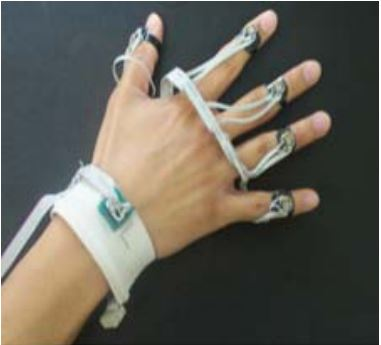
\includegraphics[scale=0.5]{images/acceleglove.JPG} 
\caption{Acceleglove system with the described sensor positions \cite{HernandezRebollar.2002}}
\end{wrapfigure}
\\To get measurements for the tilting of the hand in respect to the horizontal plane, two tilt sensors were mounted. Finally two inertial sensors for measuring the twisting of the forearm and the flexing of the wrist were utilized. This glove was intended for creating alphanumeric characters from hand positions. Recognition of hand signs was performed via a hard-wired circuitry, which mapped 80 unique combinations of sensor readings to a subset of the 96 printable ASCII characters.
\\These early systems only provided a limited amount of sensors as the electronic parts were much larger than today. This also resulted in the operation not being very user friendly. As they were developed to serve very specific applications, they were used only briefly, and never for commercial use.\\
Modern developements in this sector include \cite{Kuroda.2004,HernandezRebollar.2002,Majeau.2012}. The \textit{AcceleGlove} \cite{HernandezRebollar.2002} consists of six dual-axis accelerometers, mounted on the fingers and the back of the palm, reporting position with respect to the gravitational vector. Sensors are placed on the back of the middle phalanges, on the back of the distal phalange of the thumb, and on the back of the palm.\\
\\Kuroda et al. \cite{Kuroda.2004} introduced the \textit{StrinGlov}, which can obtains full \textit{Degrees of Freedom} of the human hand using 24 \textit{Inductcoders} and 9 contact sensors, and encodes hand postures into posture codes on its own \textit{Digital Signal Processor} (DSP). The bending angles of the fingers are measured with the \textit{Inductcoders}.\\These sensors relate the finger movement to a change in magnetic flux induced by the movement of the sensor parts that are attached to the finger. The sensor functionality is similar to the functionality of the light sensors from \cite{ThomasA.DeFanti.1977}. The 9 contact sensors, also based on magnetic fields, are put on the fingertips and on the inside of the hand to be able to measure contact between two fingertips or the fingertips and the hand. The system furthermore benefits from simple structure, which leads to low production cost. \\\\
Majeau et al. \cite{Majeau.2012} proposed a systems that uses optical flexion sensors to determine the bending angles of the fingers. The optical flexion sensors consist of a \textit{Light Emitting Diode} (LED), a photodetector and an optical fibre. The LED emits light which travels through the optical fibres. The intensity that results as the output from the fibre end is measured by the photosensor. This measuring principle also corresponds to the principle of \cite{ThomasA.DeFanti.1977}. \\Furthermore, the system is also capable of measuring the abduction of two fingers. Here, the LED is mounted to one finger and the detector to the other. The optical fiber is run from the LED down the finger to the knuckle base and then up to the detector. When abducting the two fingers, the angle at the knuckle base changes: This results in an intensity change at the detector through the loss of intensity at the curvature of the optic fiber.
The change in intensity of both measuring techniques can be mapped to corresponding hand movements.
Further readings on sensor based hand tracking systems can be found in \cite{Dipietro.2008,Sturman.1994}.
\subsection{Appearance based - Optical marker}
\label{Appearance Based Optical marker}
Optical approaches use properties of the human hand to hand to estimate the current position. The evaluation of the hand pose is usually split up into two steps. The first one is the registration of the "real" hand.\\
This is mostly done by at least one camera which is aimed at the hand. The camera then supplies a continuous stream of image data to an evaluation software. In the second step, the evaluation software tries to find key spots in the provided images. This data is then used for the search of the matching digital hand pose. The definition of the key spots for the pose matching can be achieved by several techniques.
\begin{figure}
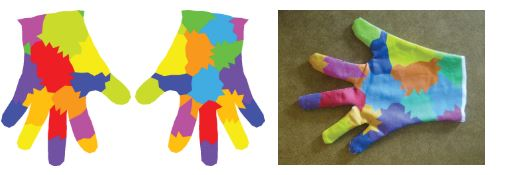
\includegraphics[width=\textwidth]{images/wang_color_glove.JPG}
\caption{Color glove setup used by Wang and Popovic  \cite{Wang.2009} }
\label{wang color glove}
\end{figure}
\\\\An example is the use of markings for finger segments as displayed in \cite{Duca.2007,Fredriksson.2008,Wang.2009}.
In the method described by Wang and Popovic \cite{Wang.2009}, a glove with a color pattern is used. The glove is segmented into ten segments, colored randomly from a pool of ten distinct colors (see Figure \ref{wang color glove}). The pattern is created by selecting twenty seed triangles on a 3D hand model that have a maximum distance to each other. The remaining triangles are assigned into patches, based on their distance to each of these seeds. Each patch is assigned one of ten colors at random. The jagged boundaries between the patches are artifacts from the low triangle count of the used hand model.
\\Algortihms that use other characteristics for tracking like texture or shading \cite{LaGorce.2008} rely on an accurate pose from a previous frame to constrain the posture search in the current frame.
When using bare hand pose estimation, two different hand poses can map to similar images. This can lead to an inaccurate pose estimation and the breakdown of the algorithm, if the wrong estimation is made.\\
The benefit of the color glove is that with the unique patch pattern, hand poses always map to distinguishable images. Therefore it can effectively recover itself at each frame without the need of a previous frame.
With the colored glove as a tracking feature, the images from the camera are prepared for a database sampling step. The database that was used consisted of 18,000 finger configurations. 
\\A distance metric between two configurations was defined as the \textit{Root Mean Square} (RMS) error between the vertex positions of the corresponding skinned hand models. With this distance metric, a low-dispersion sampling was used to draw a uniform set of samples from the over-complete collection of finger configurations.
\\The selected configurations are rendered at various 3-D orientations using a synthetic hand model at a fixed position from the virtual camera.
The camera image was then compared to the database images. This is done via a nearest neighbor lookup using a \textit{Hausdorff-like} distance \cite{Huttenlocher.1993} and penalizing the distance to the closest pixel of the same color in the other image. The resulting pose from the database can then be applied to the digital hand model.\\\\
The method presented by Fredriksson and Ryen \cite{Fredriksson.2008} also uses a color coded glove. In contrast to the fully colored glove described before, the used glove only has colored fingertips. Color markers for the palm and a colored band for the wrist are also used.
\begin{wrapfigure}[15]{r}{0.4\textwidth}
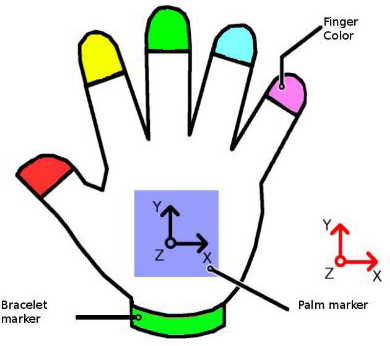
\includegraphics[width=0.4\textwidth]{images/fredrikkson_color_glove.JPG}
\caption{Color glove setup used by Fredriksson and Ryen  \cite{Fredriksson.2008} }
\label{Fredriksson color glove}
\end{wrapfigure}
The palm markers and the wrist band are used to retrieve the 3D position of the hand. The wrist marker is furthermore used to define the bounding box of the the tracking area in a calibration process. Defining a bounding greatly simplifies further image analysis operations by taking away a large amount of unneeded image data.\\
After determining position and orientation of the hand in 3D by utilizing wrist band and palm marker position, the system tracks the grip angle and the lateral tilt angle for each finger.
The grip angle is defined as the curling of the finger towards the palm. The second angle is defined as the lateral tilt angle, which measures the spread of the fingers.\\The grip angle is calculated by comparing the density of finger pixels around an estimated knuckle line. From the density, an estimation for the fingers y-axis position around an origin position at the knuckles base is made. This value is then transformed into an angle value using an inverse tangent operation.\\\\
One downside of this tracking method is that it does not incorporate the movement of the thumb. The thumb has other movement possibilities and therefore needs a different algorithmic approach. Also the approach only focuses on the the tracking of the hand data and does not implement a digital counterpart.
\subsection{Model based - Image analysis}
Hand tracking with image analysis of optical marker positions has the flaw that these markers have to be put onto the hand. Using a glove for this purpose imposes just a little bit of inconvenience, but has the drawback of not fitting every hand shape equally. Gloves also impose the problem of having to deal with hygiene when switching between users.\\The most natural way of tracking the human hand would be by simply using the properties of the human hand like skin color and shape for tracking. This would remove the need for any artificially added tracking features and has the greatest amount of comfort for the human user.
A full overview of the technological advances in this area can be found in \cite{Moeslund.2006,Moeslund.2001}. The next part will only highlight some of the main topics displayed.\\\\
As already explained before, the human hand motion leads to a large variety of shapes with many self-occlusions. This becomes even more critical when trying to reproduce the human hand pose via computer vision. Also the separation between background image information and the relevant hand information is a major topic, which is usually also the first step in the algorithmic process.\\\\
An established method for the extraction of background data was introduced by Stauffer and Grimson \cite{Stauffer.1999}. It uses the idea of representing each pixel value as a \textit{Mixture of Gaussian functions} (\textit{MoG}) and updating these pixels during run time with new \textit{Gaussian functions}.\\
The algorithm stores the mean, the variance, and the likelihood value, based on previous values, for each pixel location and distribution. 
A new input is compared to the stored mean values for each distribution at this location.\\
A result that is less than a constant times the variance declares that this pixel is part of that distribution and should be updated accordingly. For a higher value result, a new distribution is created which replaces the least probable distribution. A new input belongs to the background, if the distribution that it is part of is one of the most likely distributions.
A foreground pixel that keeps the same color over time will slowly be incorporated into the background.\\
The decision rule, whether a new pixel belongs to an existing distribution or not, can be written as \cite{Kristensen.Feb.2007}:\\
\begin{equation}
 if\ (|P_{new} −P^{d}_{mean}|\leq KP^{d}_{std})\quad then \quad P_{new}\  \in\ Distribution\ d
\end{equation}
\\Where $P_{new}$ is the new pixel value. $P^{d}_{mean}$ and $P^{d}_{std}$ are the stored mean and standard deviation of distribution \textit{d} values. \textit{K} is a constant. The convenience of this method is that it is also able to subtract background information from uncontrolled environments. This makes it possible for systems to work outside of lab conditions.
After the segmentation of foreground and background is achieved,the hand pose has to be retrieved from the left-over image data. Solutions for retireving a full set of DOF as hand pose estimation data can be split into two main categories \cite{Erol.2007}, \textit{Model-based tracking} and \textit{Single frame pose estimation}.\\\\
\textbf{Model-based tracking} refers to a top-down tracking method based on parametric models of the 3D hand shape and it's kinematic structure. The root idea here is to execute a search at each frame of an image sequence to find the pose of the shape model that best matches the features extracted from the images. A prediction based on previous motion and dynamics data from the object is set up as a base for the search. Optimization features can be incorporated, like employing a local search around the calculated prediction to produce a single best estimate at each frame. The downside of this method is the weakness of accumulating errors over longer run time periods due to occlusions and complexity of hand motion. These can be overcome by keeping track of multiple outcome hypotheses at each frame for error reduction.
\\\\
\textbf{Single frame pose estimation} in contrast to the previous method, does not utilize assumptions on time coherence. At each iteration of the search algorithm the whole data set is searched for a match.  On one side, this introduces more computational work for achieving a match. On the other side, this lowers the amount of constraints that have to be put on the user when initializing the tracker system. Furthermore, the possibly rapid motion of the human hands and fingers acts as failure factor for time coherence dependent approaches, where a single frame approach is not as vulnerable.
\section{State of the art technologies}
\label{sec:state_of_the_art}
\begin{wrapfigure}[12]{r}{0.5\textwidth}
\label{img:kinect}
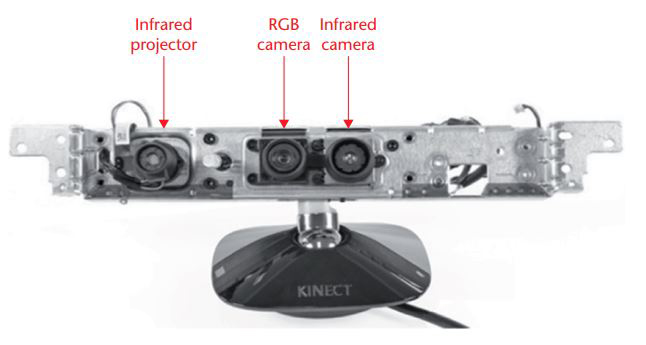
\includegraphics[width=0.5\textwidth]{images/kinnect.JPG} 
\caption{Microsoft kinect camera system with the three used sensor units \cite{Zhang.2012}}
\end{wrapfigure}
The currently most used type of system for tracking hardware is a setup of a combination of RGB and infrared sensors for imaging an depth measurement (RGB-D). The first commercial system using this technology is the \textit{ Microsoft Kinect} system \cite{Zhang.2012}. The system uses a infrared projector and an infrared sensor to measure distances in the captured scene.\\
State of the art systems that also incorporate depth sensing through infrared distance measurement are the \textit{Intel RealSense} system and the more consumer focused \textit{Leap Motion Controller}. The\textit{ Leap Motion Controller} does not supply a separate RGB sensor and does therefore only provide depth measurement data within a specific range from the device \cite{Weichert.2013}. It combines two infrared cameras with three infrared emitter LED's.
\begin{figure}[H]
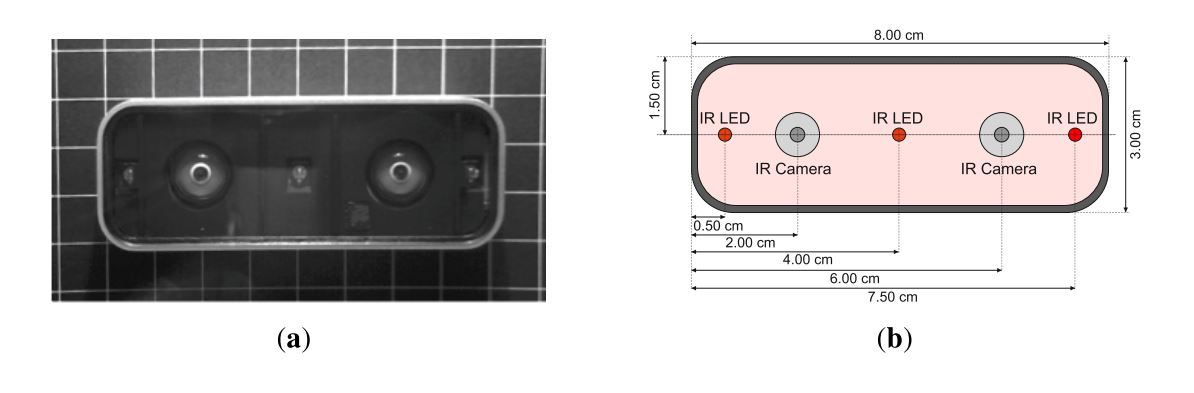
\includegraphics[width=\textwidth]{images/leapMotion.JPG}
\caption{Visualization of a (a) Real (using infrared imaging) and (b) Schematic View of the \textit{Leap Motion Controller} \cite{Weichert.2013}.}
\label{img:leapMotion} 
\end{figure}
The latest product in this category are the \textit{Intel RealSense} camera systems \cite{IntelCorporation.2018}. The Intel systems, like the\textit{ Leap Motion Controller} utilize a stereoscopic infrared system setup, and can also provide RGB sensor data, depending on the selected model.
\begin{figure}[H]
\centering
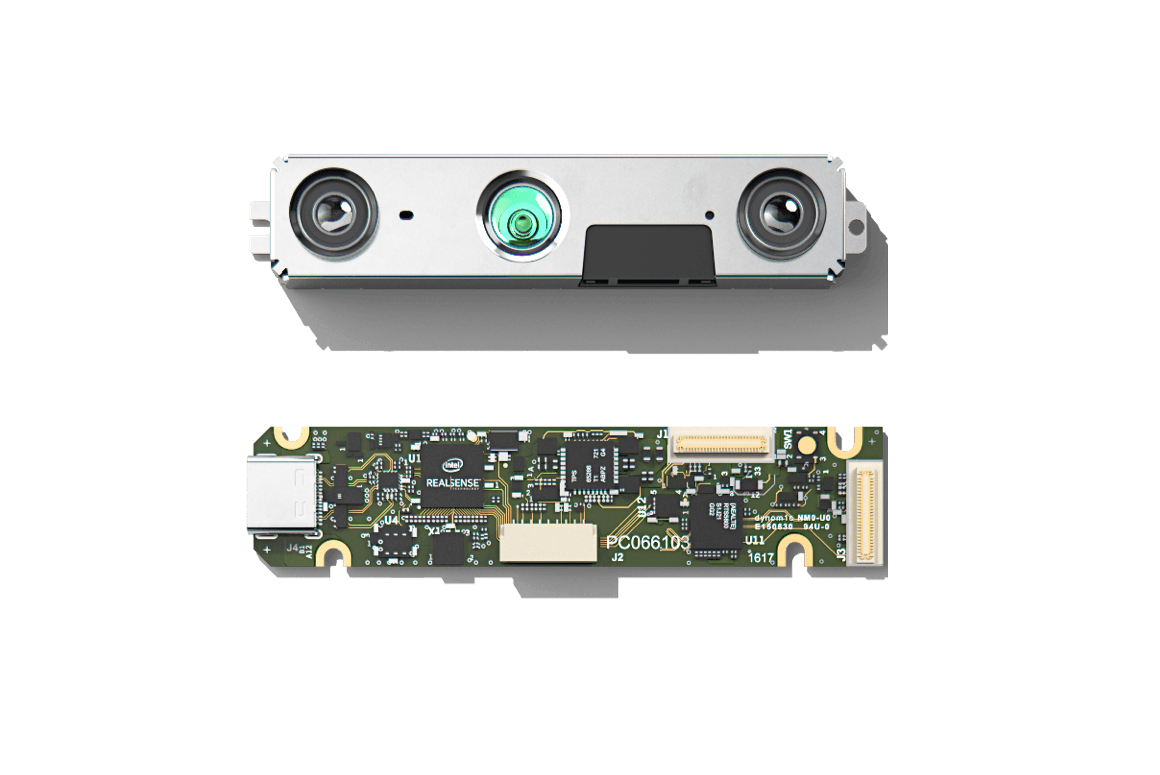
\includegraphics[width=0.6\textwidth]{images/RealSense.png}
\caption{Visualization of a \textit{Intel ReaslSense} depth module\cite{IntelCorporation.2018}}
\label{img:realsense} 
\end{figure}
The \textit{Kinect} can supply depth data at around 30 fps. It's modern descendants from Intel can supply data at frame rates of up to 90 fps. The systems provide the convenience of not having to apply any form of distinguishable marking to the surface that has to be tracked. The downside of this feature is that the devices only supply SDKs for accessing the collected data from the device. The post processing of this data needs additional sophisticated image analysis or neural network processing to figure out feature points of the tracked object from the supplied image data \cite{JamieShotton.2011,Oikonomidis.2011b}.
\\\\Image analysis of large images can be expensive for real time applications and training of new neural networks for image analysis is also time consumable. The tweaking of the network parameters and network retraining until the trained result fits the application also consume greater amounts of time. An recent approach of combining RGB-D Data and the usage of\textit{ CNNs} (Convolutional Neural Networks) to estimate hand pose and render a correct digital representaion of the hand is shown in \cite{Mueller.2017}.
\\Their approach uses two subsequently applied \textit{CNN's} to localize the hand and regress 3D joint locations. The first \textit{CNN} estimates the 2D position of the hand center in the input. The combined information of the hand position, together with the corresponding input depth value, is used to generate a normalized cropped image. This image is then fed into a second \textit{CNN} to regress relative 3D hand joint
locations in real time. Pose estimation is furthermore refined by using a kinematic pose tracking energy to achieve more accuracy, robustness and
temporal stability.
\\They also introduce a new photo-realistic data set that uses a merged reality approach to capture and synthesize large amounts of annotated data of natural hand interaction in cluttered scenes for CNN training data.